% The FYP template is designed according to NTU SCSE FYP guidelines on https://www3.ntu.edu.sg/scse/fyp/UsefulInfo/Report%20Guide.pdf.

% Credit
% Original version by Vincent Ribli
% https://www.overleaf.com/latex/templates/ntu-scse-fyp-template/kwdtcbqmjctk

% Revised by Prof Loy Chen Change
% 23 Aug 2024 - Replace SCSE with CCDS

\documentclass[pdftex, 12pt, a4paper]{report}
\usepackage{CJKutf8}

% \usepackage{ifluatex}
% \ifluatex
%   \usepackage{pdftexcmds}
%   \makeatletter
%   \let\pdfstrcmp\pdf@strcmp
%   \let\pdffilemoddate\pdf@filemoddate
%   \makeatother
% \fi
\usepackage{svg}
% \usepackage[pdftex]{graphicx}


\usepackage{newtxtext, newtxmath}
\usepackage[top=3cm, bottom=3cm, left=3.5cm, right=3cm]{geometry}
\usepackage[hidelinks]{hyperref}
\usepackage{booktabs}
\usepackage{setspace}
\usepackage{titlesec}
\usepackage{tocloft}
\usepackage{parskip}
\usepackage{amsmath}
\usepackage{amsfonts}
\usepackage[sorting=none]{biblatex}

\addbibresource{bib.bib}
\setstretch{1.5}
\setlength{\cftfigindent}{0pt}
\setlength{\cfttabindent}{0pt}
\renewcommand{\cftdotsep}{1}

% change the following
\title{\uppercase{Transformers and Attention Mechanisms}}
\newcommand\fypcode{SCSE8338}
\author{
\begin{CJK*}{UTF8}{bkai}
110550079 林伯蔚 \\
110550159 劉秉庭
\end{CJK*}
}
\date{2024/12}
\newcommand\degree{Bachelor of Engineering in Computer Science}

\begin{document}
\makeatletter
\begin{titlepage}
\begin{center}

\uppercase{\textbf{\large{Mathematical foundations of machine learning, Final Report}}}
\\[7cm]

\uppercase{\textbf{\large{\@title}}}

\vfill
\@author
\\[3cm]

% Mathematical foundations of machine learning, Final Report

\@date

\end{center}
\end{titlepage}
\makeatother
% \makeatletter
\begin{titlepage}
\begin{center}

\uppercase{\textbf{\large{Nanyang Technological University}}}
\\[6cm]

\uppercase{\textbf{\fypcode \\[0.3cm]\@title}}

\vfill

Submitted in Partial Fulfilment of the Requirements\\
for the Degree of \degree\\
of the Nanyang Technological University
\\[0.8cm]
by
\\[0.8cm]

\@author
\\[2cm]

\end{center}

College of Computing and Data Science\\
\@date
\end{titlepage}
\makeatother

% \setcounter{page}{1}
% \pagenumbering{roman}

% \chapter*{Abstract}
\addcontentsline{toc}{chapter}{Abstract}

Lorem ipsum dolor sit amet, consectetur adipiscing elit. Morbi lobortis id nunc a maximus. Nam vitae pellentesque elit. Ut lacus arcu, consectetur at erat sed, sollicitudin suscipit dolor. Sed pharetra, ipsum id volutpat dictum, lacus ante hendrerit mauris, ac tristique orci dui quis dolor. Suspendisse dictum magna vitae fermentum maximus. Quisque vulputate urna id turpis pulvinar suscipit. Praesent sit amet finibus ante. Nullam dignissim sapien ac dolor elementum accumsan. In fermentum tellus eu velit ullamcorper pellentesque id eu eros. Phasellus erat elit, luctus eleifend urna eu, consequat fringilla nisl. Aenean convallis mattis libero, eu dignissim ligula mollis at. Cras pharetra imperdiet risus, in placerat sem ultrices ultrices. Donec eget augue condimentum, efficitur nunc vel, fermentum lacus.
% \chapter*{Acknowledgments}
\addcontentsline{toc}{chapter}{Acknowledgments}

The writer uses this section to thank all those he or she is indebted for guidance, financial or any other assistance rendered during the course of the project.




\pagebreak
\addcontentsline{toc}{chapter}{Contents}
\tableofcontents

% \pagebreak
% \addcontentsline{toc}{chapter}{List of Tables}
% \listoftables

% \pagebreak
% \addcontentsline{toc}{chapter}{List of Figures}
% \listoffigures

\cleardoublepage
\pagenumbering{arabic}

\chapter{Introduction}

\section{Background}

\textbf{Transformer} is a deep learning architecture proposed in the 2017 paper \textit{Attention Is All You Need} \cite{vaswani2017attention}, developed initially for machine translation. The transformer architecture has literally transformed the whole deep learning community since its debut, with its multiple advantages, including:

\begin{enumerate}
    \item \textbf{Efficacy}: Transformers utilize \textit{multi-head attention mechanism}, which effectively captures global information while processing data.
    \item \textbf{Efficiency}: The design of Transformer (discarding recurrent networks) allows significant parallelization, which greatly speeds up model training and evaluation.
\end{enumerate}

To date, Transformer has not only gained tremendous success in NLP tasks (e.g. GPT-4 \cite{achiam2023gpt}), but has also been applied to modalities beyond text, including image/video generation (e.g. Sora \cite{videoworldsimulators2024}), computer vision (e.g. ViT \cite{dosovitskiy2020image}), and more. Here, we merely focus on NLP tasks for simplicity.

\section{Related Works}

In essence, the transformer architecture incorporates multiple past innovations, including attention mechanism, layer normalization, residual connection, etc.

Prior to the transformer architecture, attention mechanisms were primarily employed within sequence-to-sequence models \cite{bahdanau2014neural}. However, these attention mechanisms were typically constrained by the sequential processing imposed by RNNs, which severely limited opportunities for parallelization. In contrast, the transformer model \cite{vaswani2017attention} replaces recurrence with a self-attention mechanism. This innovative approach enabled parallel computation across the entire input sequence, leading to substantial improvements in training efficiency and scalability. 

Layer normalization is proposed in \cite{ba2016layer} to address the problems of batch normalization and acts as a method for normalization in RNNs. Residual networks, first appearing in \cite{he2016deep}, aim to solve training issues of deep neural networks, especially in CNNs. Both layer normalization and residual connections enable a more stable training process for transformers.

\section{Transformer Overview} \label{sec:transformer_overview}

The transformer architecture mainly consists of two components: (1) \textbf{embedding layers} (2) \textbf{transformer blocks}. An embedding layer maps input tokens (or simply, \textit{words}) to numerical representations, or vice versa. That is, input words are converted to numerical vectors (embeddings) for further processing. And after all calculations, those embeddings are converted back to textual data. The transformer blocks constitute the core of the overall architecture. A transformer block is composed of the following:

\begin{itemize}
    \item \textbf{an attention layer},
    \item \textbf{a feedforward layer},
    \item \textbf{layer normalizations (layer norms)}, and
    \item \textbf{residual connections}.
\end{itemize}

Figure \ref{fig:tranformer_atchitecture} illustrates the transformer architecture globally. In the following sections, we will first introduce the \textbf{attention mechanism} in Chapter \ref{chap:attention}. The other ingredients of the transformer block will be covered in Chapter \ref{chap:transformer}.

\begin{figure}
    \centering
    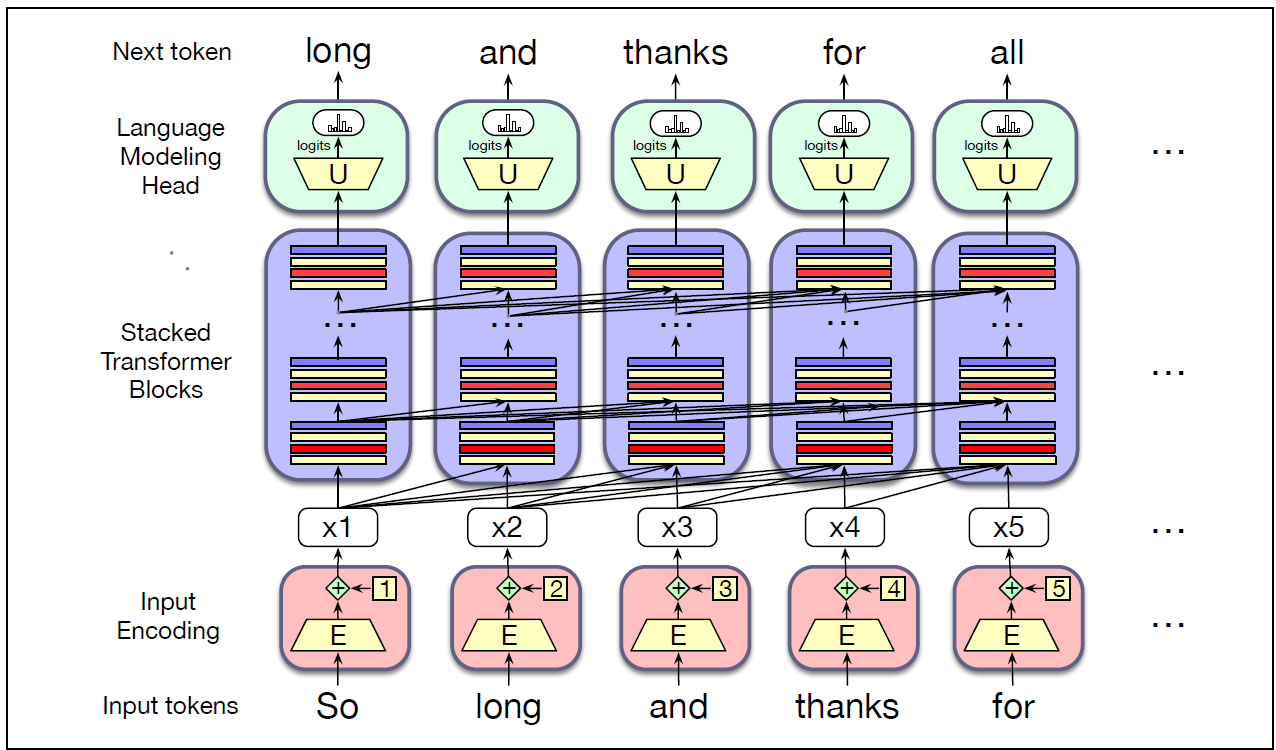
\includegraphics[width=1\linewidth]{fig/transformer_architecture.png}
    \caption{A (decoder-only) transformer model illustration for text generation \cite{jm3}.}
    \label{fig:tranformer_atchitecture}
\end{figure}
\chapter{Attention} \label{chap:attention}

\section{Overview}

A core challenge in Natural Language Processing (NLP) is designing machines capable of understanding human language. Various algorithms have been developed to address this, including recurrent neural networks (RNNs) and more sophisticated architectures like Long Short-Term Memory (LSTM) networks. These models process input tokens sequentially, updating an internal "hidden state" to maintain context. However, because a single hidden state is used to represent all past information, subtle nuances in the language can be lost.

Attention mechanisms offer an alternative approach. Instead of a single hidden state, each token is assigned its own unique representation, and information is selectively passed between these representations. This allows for better preservation of contextual information for future token predictions. Furthermore, the calculations involved in attention mechanisms are highly parallelizable, which enables the training of larger models on more extensive datasets.

% Recurrent neural networks (RNN) and more advanced architectures like Long short-term memory (LSTM) have the ability to \textit{remember} history states while handling the current input token. However, since a single hidden state is shared by all past information, nuances may not be captured precisely. \textbf{Attention} mechanism was developed to address such weaknesses: With attention mechanism, information of tokens are shared between one another, such that each token is exclusively represented by its own hidden state. This means that contextual information is better preserved for future token inferences.

% For example, suppose that we try to capture the meaning of the words \textit{toy car}. Recall that each word is embedded as a vector while being processed, and words with similar meanings are embedded closely. The embedding for \textit{car} should be correlated to vectors associated with \textit{large}, \textit{gasoline-driven} vehicles. With attention mechanism, a contextual embedding is calculated based on the past token \textit{toy}, such that the updated embedding for \textit{car} is no longer correlated to large things but smaller models. In general, attention mechanism can encode much richer information than just a single word in the context, and can determine the relative importance of each component that is attended to.

\section{Attention Mechanism}

Having established that attention mechanisms facilitate information flow between word representations, two key questions emerge:

\begin{enumerate}
    \item From which words should information be retrieved?
    \item What specific information should be transferred?
\end{enumerate}

The answers to these questions form the foundation of attention mechanisms. In the subsequent section, we will begin by exploring the \textbf{single-head attention mechanism}.

\subsection{Single-Head Attention Mechanism}

\begin{figure}
    \centering
    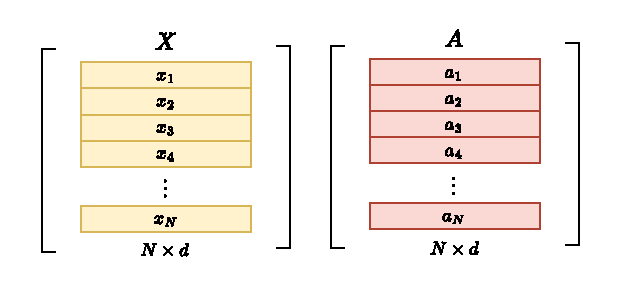
\includegraphics[width=1\linewidth]{fig/X_A.pdf}
    \caption{Left: $N$ input $d$-dimensional vectors stacked into $X$. Right: $N$ attention vectors for each input vector, stacked into $A$. Note that $X$ and $A$ have the same size.}
    \label{fig:X}
\end{figure}

A single-Head attention mechanism operates on sequences of tokens, where a \textbf{token} typically represents a word, sub-word unit, or character. These tokens are transformed into dense vector representations within a $d$-dimensional space, commonly referred to as \textbf{embeddings}. For an input sequence of $N$ tokens, $\{x_i\}_{i=1}^N$, these embeddings are stacked to form an $N \times d$ matrix, denoted as $X$. The goal for single-head attention is to calculate an \textit{attention matrix} $A$ for $X$ such that the $i$-th row of $A$ contains new information for the $i$-th input vector $x_i$: Our understanding of the inputs $X$ is then updated to

$$
X' = X+A.
$$

Figure \ref{fig:X} visualize the input $X$ and the attention matrix $A$.

Intuitively, the calculations for $A$ consists of the following four steps:

\begin{enumerate}
    \item \textbf{Tokens ask}: Who has information for me? (\textit{Query})
    \item \textbf{Tokens reply}: Here is my answer! (\textit{Key})
    \item \textbf{Tokens determine}: I would like to share this piece of information! (\textit{Value})
    \item \textbf{Collect} the pieces of information shared, and \textbf{weight} them according to how well a response answers a query.
\end{enumerate}

To shed more light on the first two steps, consider the below input sequence: \textit{an interesting report} (embedded word-by-word as $(x_1, x_2, x_3)$). Imagine that for the word \textit{report}, it asks: \textit{Any adjectives in front of me?}, and the word \textit{interesting} answers: \textit{I am!}. To capture this question-answering  process mathematically, the question is encoded into a vector $q$ called \textit{query}, via a weight matrix $W^Q$ with size ${d \times d_k}$, where $q_3 = x_3  W^Q.$ Similarly, the answer is encoded in another vector $k_2$ called \textit{key}, via some weight matrix $W^K$ of the same size as $W^Q$, where $k_2 = x_2 W^K$.

To measure how well a key $k_j$ answers a query $q_i$, we compute the dot product between them, i.e., $q_i \cdot k_j$. If two vectors are similar \textit{in direction}, the dot product between them should be relatively large. In this sense, the dot product $q_3 \cdot k_2$ should be large, since $k_2$ is an exact answer to $q_3$. The weight matrices $W^Q$ and $W^K$ are parameters to be trained, such that input vectors can be mapped to good questions and keys that align with the above intuition. In general, the calculations of queries, keys, and determining the similarities of queries and keys, are done in a single matrix multiplication respectively. 
% The computations are illustrated in Figure \ref{fig:XWQ}, \ref{fig:XWK}, and \ref{fig:QK^T}.

% \begin{figure}
%     \centering
%     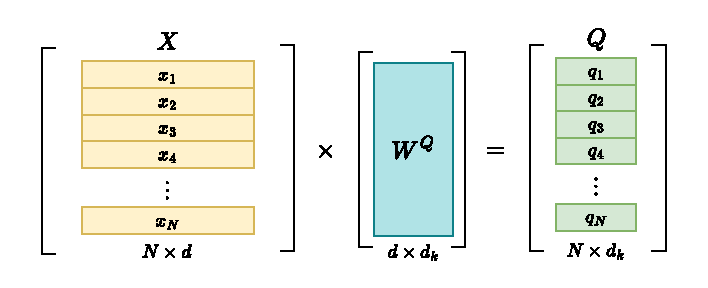
\includegraphics[width=1\linewidth]{fig/XWQ.pdf}
%     \caption{Compute queries $Q$ from input $X$ via weight $W^Q$}.
%     \label{fig:XWQ}
% \end{figure}

% \begin{figure}
%     \centering
%     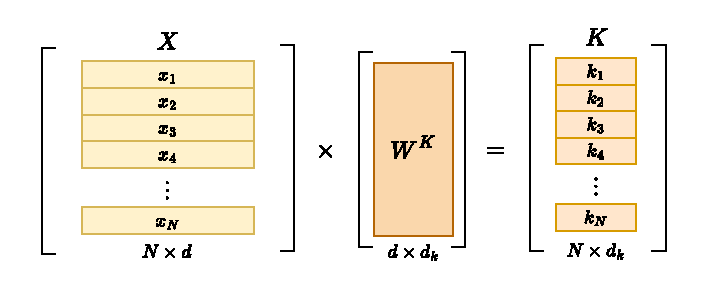
\includegraphics[width=1\linewidth]{fig/XWK.pdf}
%     \caption{Compute keys $K$ from input $X$ via weight $W^K$}
%     \label{fig:XWK}
% \end{figure}

As for the information that a token is to share, it is likewise encoded into a vector $v=xW^V$ called \textit{value}, where $W^V$ is yet another weight matrix with size $d \times d_v$. Since the word \textit{interesting} properly answers the query from \textit{report} (i.e., $q_3 \cdot k_2$ is large), the information passed from \textit{interesting} to \textit{report} should be ``significant'', compared to that passed from \textit{an} to \textit{report}. We capture this ``significance'' of information passed to \textit{report} by regarding  $\{q_3 \cdot k_i\}_{i=1}^4$ as weights, and converting them into a probability distribution via \textit{softmax}: For $i \in \{1, 2, 3, 4\}$, we have $\alpha_{j3} =  \text{softmax}(\{q_3 \cdot k_i\}_i)_j$. The \textit{attention vector} $a_3$ for the word \textit{report} is therefore a weighted sum of $\{v_i\}_{i=1}^4$, where 
$$
a_3 = \sum_{i=1}^{4} \alpha_{i3}v_i.
$$
Repeat this process for all input words, we would obtain the attention matrix $A$! The calculations for \textit{query}, \textit{key} and \textit{value} are illustrated in Figure \ref{fig:XWQ_XWK} and \ref{fig:XWV}, and dot product computations are illustrated in Figure \ref{fig:QK^T}. The single-head attention mechanism can be summarized by a well-known, compact equation:
\begin{equation}\label{eq:1}   
    A = \text{Attention}(Q, K, V) = \text{softmax}\bigg({\frac{QK^T}{\sqrt{d_k}}}\bigg)V, 
\end{equation}
where $\sqrt{d_k}$ is introduced for numerical stability.

\begin{figure}
    \centering
    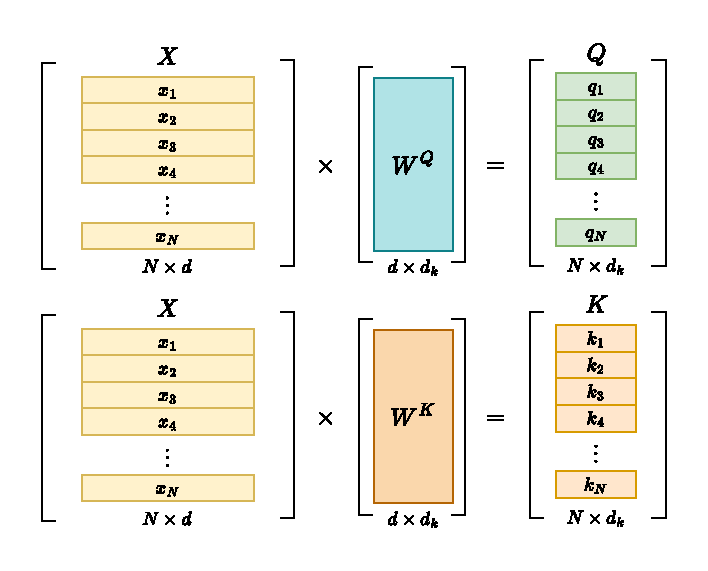
\includegraphics[width=1\linewidth]{fig/XWQ_XWK.pdf}
    \caption{Compute queries $Q$ for input $X$ via weight $W^Q$, and compute keys $K$ for input $X$ via weight $W^K$.}
    \label{fig:XWQ_XWK}
\end{figure}

\begin{figure}
    \centering
    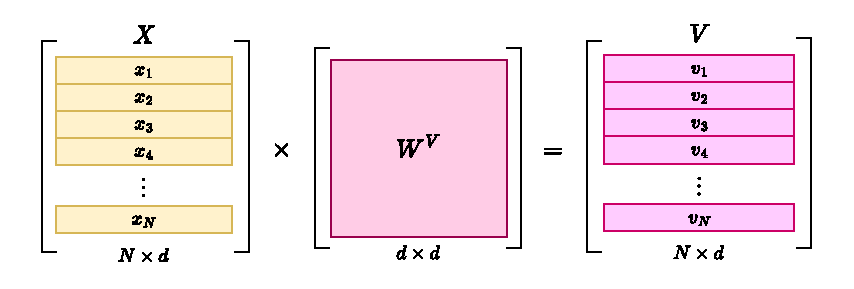
\includegraphics[width=1\linewidth]{fig/XWV.pdf}
    \caption{Compute values $V$ for input $X$ via weight $W^V$. Note that for single-head attention, we must take $d_v = d$ in order for $A$ to match the size of $X$.}
    \label{fig:XWV}
\end{figure}

\begin{figure}
    \centering
    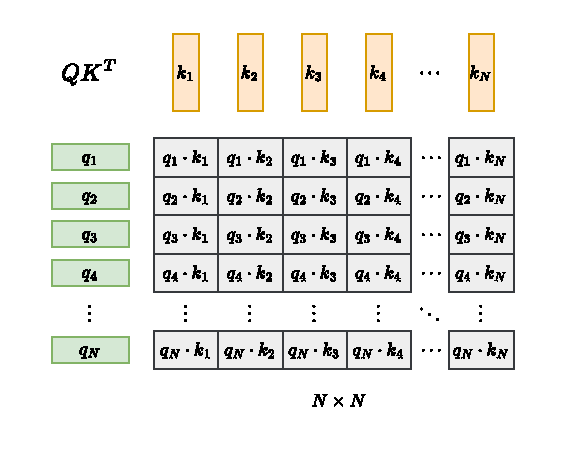
\includegraphics[width=0.8\linewidth]{fig/QK-T.pdf}
    \caption{Compute the similarity (dot product) between all pairs of queries and keys.}
    \label{fig:QK^T}
\end{figure}

\subsection{Multi-Head Attention Mechanism}

A single \textbf{attention head}, as described by Equation \eqref{eq:1}, captures a specific information flow pattern within the context of a sentence. However, natural language exhibits a wide variety of such patterns. Consequently, Transformer models in fact use multi-head attention to combine multiple attention heads. Each head has its own set of weight matrices ($W^Q_i$, $W^K_i$, and $W^V_i$), allowing the input ($X$) to be projected into separate query, key, and value embeddings for each head.

A naive approach to combining $h$ single-head attention outputs would be to sum them: $A = \sum_i A^{(i)}$, where $A^{(i)}$ is the output of $i$-th head. However, this method becomes parameter-inefficient because the weight matrix $W^V_i$, with dimensions $d \times d_v$ (where $d_v = d$ for single-head attention), is substantially larger than $W^Q_i$ and $W^K_i$, both of which have dimensions $d \times d_k$ (where $d_v = d \gg d_k$). This would lead to an unacceptably large number of parameters in the multi-head attention mechanism. To address this, a more parameter-efficient approach was introduced in the original Transformer paper \cite{vaswani2017attention}.

The multi-head attention mechanism refines the process by decomposing the $d \times d$ matrix $W^V_i$ of each head into a product of two smaller matrices: a matrix $W^V_i$ of size $d \times d_v$ and a matrix $W^O_i$ of size $d_v \times d$, where $d_v < d$. While the result of the product has dimensions $d \times d$, this decomposition reduces number of parameters to represent the matrix, but its rank is reduced as well, limiting the fitting power of the model. 

The original Transformer paper maintains the value calculation for each head as $XW^V_i$. With $W^V_i \in \mathbb{R}^{d \times d_v}$, the output of each head has a shape of $N \times d_v$. To obtain an output with dimensions $N \times d$ for the multi-head attention, the outputs from each head (each with dimensions $d \times d_v$) are concatenated horizontally to form a matrix of size $d \times hd_v$. The matrices $W^O_i \in \mathbb{R}^{d_v \times d}$ from each head are then concatenated vertically to produce a matrix $W^O \in \mathbb{R}^{hd_v \times d}$.  Finally, the concatenated head outputs are multiplied by $W^O$ to obtain the final output of the multi-head attention. This process is illustrated in Figure \ref{fig:concat_project_A}.

In summary, multi-head attention enhances the standard attention mechanism by allowing the model to capture multiple different relationships between words in a sentence. It does this by using multiple attention heads with separate weight matrices that project the input into different subspaces, allowing for parallel processing of different aspects of the input. Then, through concatenation and projection the output from each head is combined into a single representation.

% Let $A^{(i)}$ denote the attention matrix calculated from the $i$-th head, and consider there are in total $h$ heads. A naive way to combine all the attention matrices is by summing them up: $A = \sum_i A^{(i)}$. However, a parameter-efficient method is proposed in the original paper \cite{vaswani2017attention}: We concatenate all the attention matrices, resulting in a $N \times hd_v$ matrix, and then apply a transformation $W^O$ of size $hd_v \times d$ on it to map the target matrix back to size $N \times d$ (which matches the size of $X$). This procedure is illustrated in Figure \ref{fig:concat_project_A}. 

% Why this method saves parameters? The naive way takes $p_0 = d \times d$ parameters for $W^V$ in each head (recall that $d_v=d$ for single-head attention). However, for the parameter-efficient method, we can actually choose $d_v < d$ as long as $hd_v > d$. In practice, we have $d_v = d/h$, and thus there is only $d \times d_v = p_0/h$ parameters per $W^V$. As a side note, the dimensions prescribed in the original paper \cite{vaswani2017attention} is: $(d, d_k, d_v, h) = (512, 64, 64, 8)$.

\begin{figure}
    \centering
    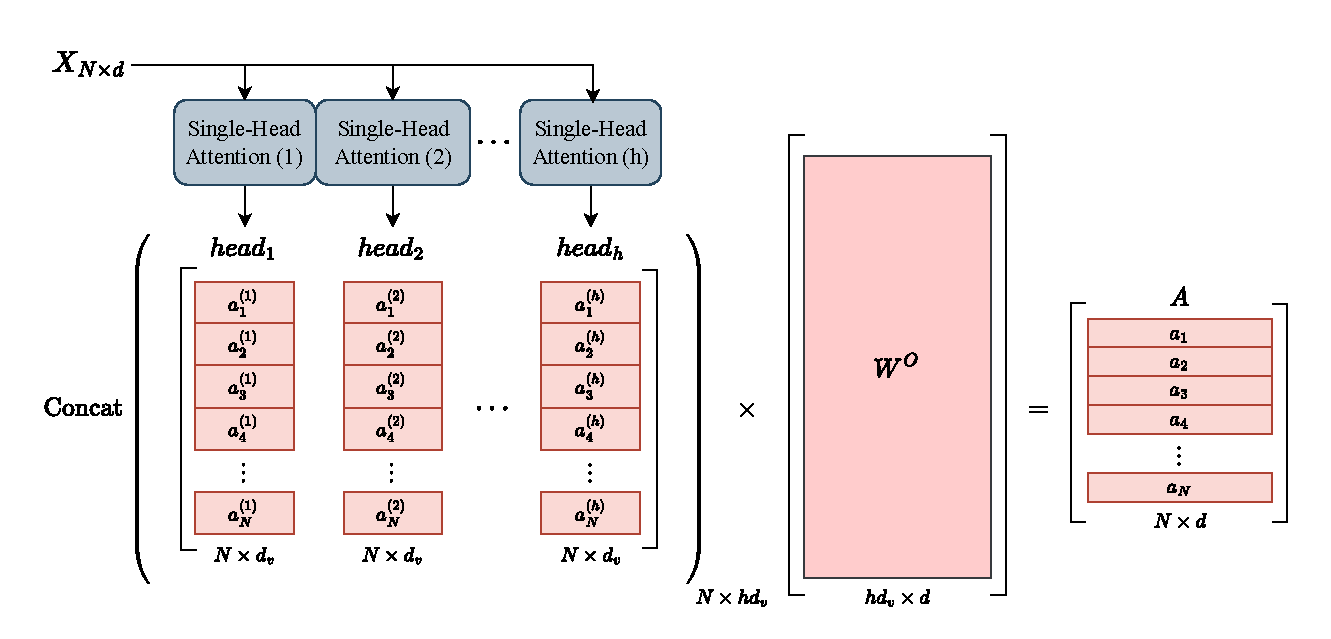
\includegraphics[width=1\linewidth]{fig/concat_project_A.pdf}
    \caption{A parameter-efficient method to accumulate all the attention heads.}
    \label{fig:concat_project_A}
\end{figure}

\chapter{Transformer} \label{chap:transformer}

We already have a glimpse of the architecture of transformers in Section \ref{sec:transformer_overview}. In this chapter, we will introduce the remaining components of transformer blocks. Figure \ref{fig:encoder_decoder} gives a close look into a transformer block.

\begin{figure}
    \centering
    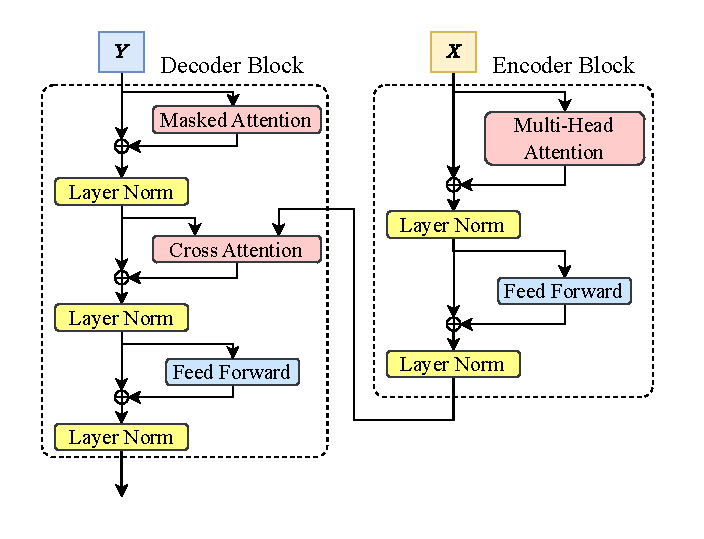
\includegraphics[width=0.8\linewidth]{fig/encoder_decoder.pdf}
    \caption{Transformer blocks. More specifically, they are an encoder block and a decoder block, which are explained in Section \ref{sec:encoder_decoder}.}
    \label{fig:encoder_decoder}
\end{figure}

% As a quick recap, a transformer consists of embedding layers and transformer blocks, where the latter have four components:

% \begin{itemize}
%     \item \textbf{an attention layer},
%     \item \textbf{a feedforward layer},
%     \item \textbf{normalization layers (layer norms)}, and
%     \item \textbf{residual connections},
% \end{itemize}

\section{Feedforward Layer}

The \textbf{feedforward layer} in transformer blocks is a fully-connected 2-layer neural network with ReLU activation, which can be written as
$$
\text{FFN}(x) = \max(0, xW_1+b_1)W_2 + b_2,
$$
where $W_1 \in \mathbb{R}^{d\times d_{ff}}$ and $W_2 \in \mathbb{R}^{d_{ff}\times d}$. (In the original paper \cite{vaswani2017attention}, the authors chose $d_{ff} = 2048 = 4d$.)
% In practice, the choice of $d_{ff}$ is often approximately $4d$. 
Feedforward layers add non-linearity into the transformer architecture, and extend the information captured by attention mechanism. Note that the weights are shared across inputs, which means that the calculations here are independent among input tokens.

\section{Layer Normalization (Layer Norm)}

In transformer blocks, \textbf{layer normalization} performs normalization on \textit{each input embedding}: Given an input embedding $x = (\chi_1, \cdots, \chi_d)$, layer normalization calculates the following:
\begin{equation}
\begin{aligned}
    \mu &= \sum_{i=1}^d \chi_i, \\
    \sigma &= \sqrt{\frac{1}{d}\sum_{i=1}^d(\chi_i - \mu)^2}, \\
    \chi_i &\leftarrow \gamma_i\frac{\chi_i - \mu}{\sigma} + \beta_i,
\end{aligned}
\end{equation}
where $\gamma$ and $\beta$ are parameters. Normalization is adopted to improve training performance, say, prevent gradient underflow/overflow. Note that the normalization process is performed \textit{feature-wise}, but not on the whole input sequence. This ensures that each feature (input embedding) remains its independence in terms of the information it captures. Finally, trainable parameters $\gamma = (\gamma_1, \cdots, \gamma_d)$ and $\beta = (\beta_1, \cdots, \beta_d)$ are introduced to restore the representational capacity of normalized embeddings, by learning a suitable scale and shift for each feature (i.e., each of the $d$ dimensions).

\section{Residual Connection}

A \textbf{residual connection} is a shortcut connection added to a neural network that bypasses one or more layers, which eases the problem of gradient vanishing. For example, consider a 2-layer feedforward network $\mathcal{N}$: $L_1(x) = xW_1 + b_2, L_2(x) = xW_2 + b_2$, and the output of this network is $y = L_2(L_1(x))$. Adding residual connection transforms the output into $y_{res} = L_2(L_1(x)) + L_1(x)$. To see why gradients might vanish, consider the following equations:
\begin{align*}
  \frac{\partial y}{\partial W_1} &= \frac {\partial y}{\partial L_2} \frac {\partial L_2}{\partial L_1} \frac {\partial L_1}{\partial W_1}, \tag{*} \label{eq:3.3.1} \\
  \frac{\partial y_{res}}{\partial W_1} &= \underbrace{\frac {\partial y_{res}}{\partial L_2} \frac {\partial L_2}{\partial L_1} \frac {\partial L_1}{\partial W_1}}_{\text{Vanish!}} + \frac {\partial y_{res}}{\partial L_1} \frac {\partial L_1}{\partial W_1}. \tag{**}\label{eq:3.3.2} \\
\end{align*}    
The original gradient (\ref{eq:3.3.1}) for $\mathcal{N}$ only involves a multiplicative term, which might be extremely small due to continual multiplications. In contrast, the addition of $\frac{\partial y_{res}}{\partial L_1} \frac {\partial L_1}{\partial W_1}$ in (\ref{eq:3.3.2}) from the residual connection is capable of mitigating this issue. The $\oplus$ in Figure \ref{fig:encoder_decoder} indicate residual connections in transformers.

\section{Encoder and Decoder Block} \label{sec:encoder_decoder}

\begin{CJK*}{UTF8}{bkai}
Inside the transformer architecture, there are two types of transformer blocks: encoder and decoder. Take a machine translation task for example. (Recall that transformer was originally proposed for translation in \cite{vaswani2017attention}.) Suppose we would like to translate ``你好嗎?" into English. An \textbf{encoder} is responsible for \textit{encoding} the whole 
sentence ``你好嗎?". A \textbf{decoder} then utilizes the information learned from the encoder, and 
sequentially outputs the translated sentence ``How are you?". Figure \ref{fig:example_translation} demonstrates this process, and Figure \ref{fig:encoder_decoder} shows the respective components of a encoder and a decoder. There are two variants of attention mechanism behind this encoder-decoder architecture: \textbf{masked attention} and \textbf{cross attention}. Details follow.
\end{CJK*}

\begin{figure}
    \centering
    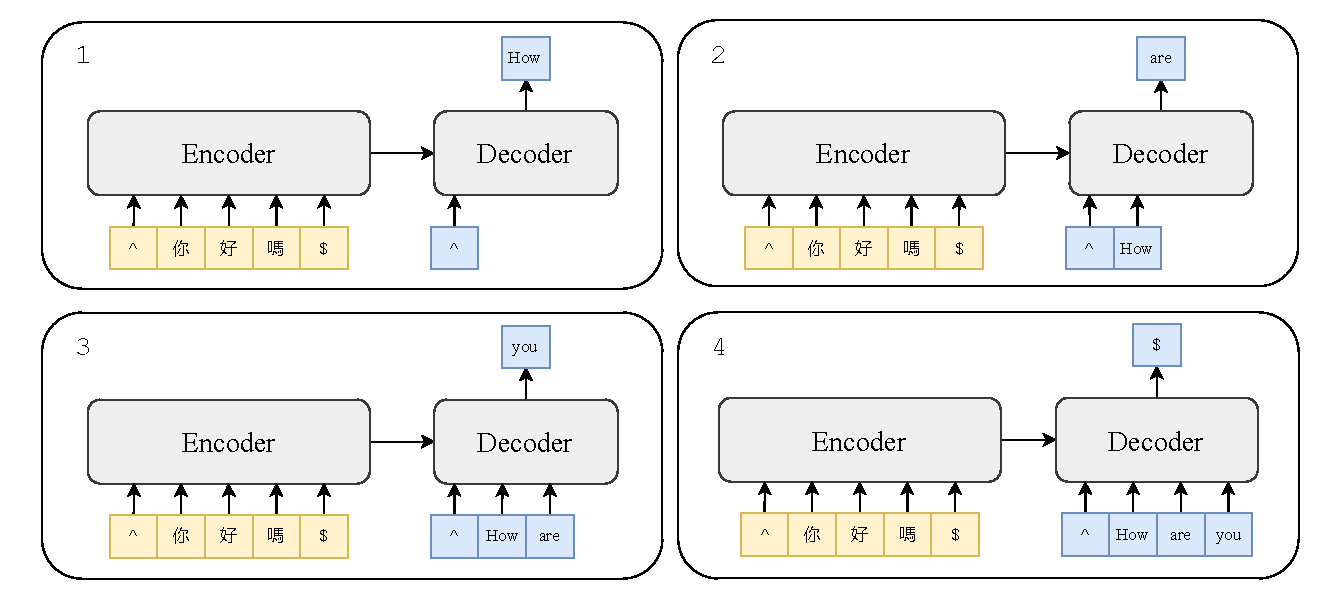
\includegraphics[width=1\linewidth]{fig/example_translation.pdf}
    % \includesvg[width=1\linewidth]{fig/example_translation.svg}
    \caption{Chinese-English translation example, with encoder and decoder blocks.}
    \label{fig:example_translation}
\end{figure}

\subsection{Masked Attention}

Ideally, each input dimension of a decoder should be able to output (predict) the \textit{next} token from its position. If the ordinary attention mechanism is applied (Figure \ref{fig:QK^T}), tokens are able to attend to \textit{future} information, which makes decoding the \textit{next} word trivial! Therefore, in the masked attention mechanism, the upper-triangular portion of $QK^T$ (the \textit{future} information) is ``masked" by $-\infty$, which essentially becomes $0$ after softmax is applied. Figure \ref{fig:masked_attention} illustrates the masked $QK^T$. It is worth mentioning that masking is more relevant to the \textit{training phase} than it would be when transformers are used in production (say, in translating texts) \cite{3b1b}.

\begin{figure}
    \centering
    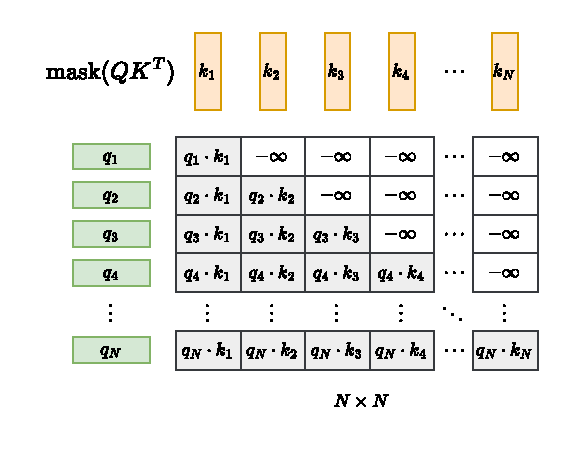
\includegraphics[width=0.8\linewidth]{fig/masked_attention.pdf}
    \caption{Masked attention.}
    \label{fig:masked_attention}
\end{figure}

\subsection{Cross Attention}

How decoders retrieve information from encoders? In the original attention mechanism, all query, key and value come from a single block (e.g. an encoder block). To allow information flows from encoders to decoders, we simply let \textit{decoders query encoders}: The queries $Q$ is from a decoder, and the keys $K$ and values $V$ are from an encoder, as shown in Figure \ref{fig:cross_attention}.

\begin{figure}
    \centering
    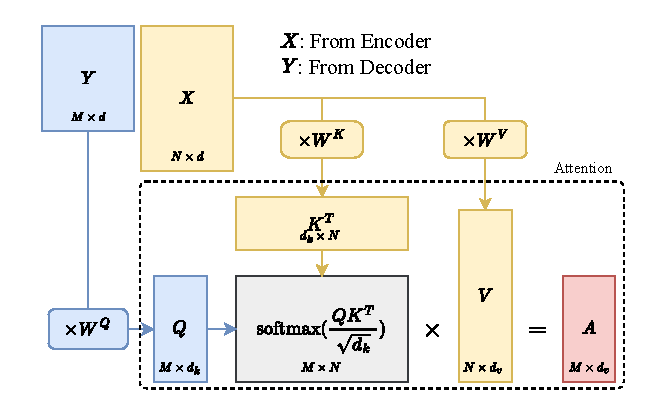
\includegraphics[width=0.8\linewidth]{fig/cross_attention.pdf}
    \caption{Cross attention.}
    \label{fig:cross_attention}
\end{figure}

\section{Embedding Layers}

As briefly sketched in Section \ref{sec:transformer_overview}, embedding layers convert words to vectors and the other way around. We can divide the embedding layers into two categories: \textbf{input embedding layer} and \textbf{output unembedding layer}.

\subsection{Input Embedding Layer}

Each transformer has an input embedding layer, which encodes the following aspects of input words: (1) \textbf{word meanings} (2) \textbf{word positions}. 

For (1), the input word $w$ is first \textbf{one-hot encoded} according to its index in the vocabulary $V$ (i.e., all the words that machines recognize). Suppose $w$ is the $16^{\text{th}}$ word in $V$. Then it would be encoded as $v = (\underbrace{0, \cdots, 0}_{15}, 1, \underbrace{0, \cdots, 0}_{|V|-16})$. Next, the one-hot vector $v$ is multiplied by the $|V|\times d$ \textbf{embedding matrix} $E$, which contains the initial representations for each word in $V$. In practice, $E$ is often pre-trained elsewhere, but not randomly initialized.

For (2), the goal is to encode each possible position of a word in a sequence into some vector of $d$ dimensions. For position $pos$, its encoding $PE(pos)$ is defined as:
\begin{align*}
    PE(pos, 2i) &= sin(pos/10000^{2i/d}), \\
    PE(pos, 2i+1) &= cos(pos/10000^{2i/d}),
\end{align*}
where $0 \le i \le \lfloor d/2 \rfloor$ is the dimension and $10000$ is a pre-defined constant. This encoding is proposed due to the following advantages:

\begin{itemize}
    \item Each position is \textbf{uniquely} encoded, and the model can extrapolate to sequence lengths \textbf{longer} than the ones encountered during training.
    \item It captures \textbf{relative positions} in the following sense: For a fixed offset $k$, $PE(pos + k)$  can be represented as a linear function of $PE(pos)$.
\end{itemize}

To combine (1) and (2), we simply sum them up: The final embedding of $w$ is $e_w := vE + PE(pos_w)$. This layer is summarized in Figure \ref{fig:embedding}.

\begin{figure}
    \centering
    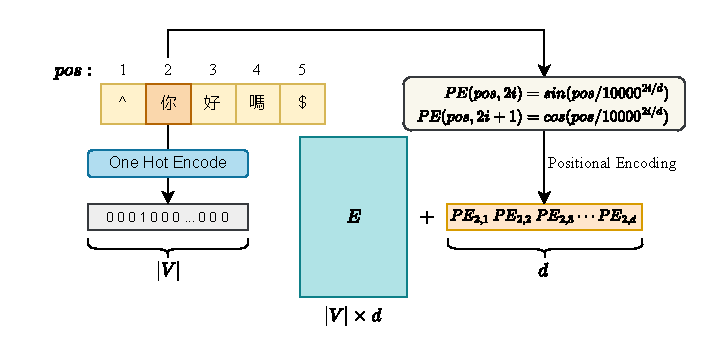
\includegraphics[width=0.9\linewidth]{fig/embedding.pdf}
    \caption{Input embedding layer.}
    \label{fig:embedding}
\end{figure}

\subsection{Output Unembedding Layer}

Each transformer also has an unembedding layer, to map the inner representations of words in a transformer to something we can more easily handle. An \textbf{unembedding matrix} $U$ of size $d \times |V|$ is multiplied to the output $Y$ of the final decoder block to generate the unembedded vectors $Y'$ (called \textit{logits}), i.e., $Y' := YU$. A softmax is then applied to the last row of $Y'$, converting its elements into a probability distribution for further processing (e.g. sampling). In practice, we may choose $U = E^T$, which is the transpose of the \textit{embedding matrix} for parameter-saving. Figure \ref{fig:unembedding} illustrates the whole process.

\begin{figure}
    \centering
    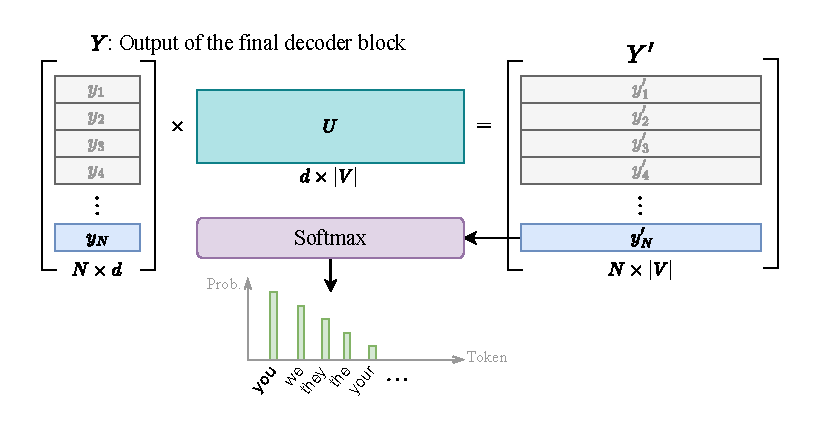
\includegraphics[width=1\linewidth]{fig/unembedding.pdf}
    \caption{Output unembedding layer.}
    \label{fig:unembedding}
\end{figure}

\section{Challenges and Conclusion}

Transformers face a few challenges, below are two prominent ones:

\begin{itemize}
    \item \textbf{Quadratic dependency on input length $d$}: As can be seen in Figure \ref{fig:QK^T}, this problem is inherent to the attention mechanism and prevents transformers from having large context window.
    \item \textbf{Interpretability}: Interpreting neural networks have always been a tough task, while transformer-specific interpretability \cite{mohebbi-etal-2024-transformer-interpret} raises even more challenges.
\end{itemize}

Eventually, this chapter is concluded with Figure \ref{fig:transformer}.


% \section{Conclusion}

% We have introduced all the ingredients in transformers. To sum up, we remark that a typical transformer consists of $L$ encoder and $L$ decoder blocks, where $L=6$ is chosen in \cite{vaswani2017attention}. This chapter is concluded with Figure \ref{fig:transformer}.

\begin{figure}
    \centering
    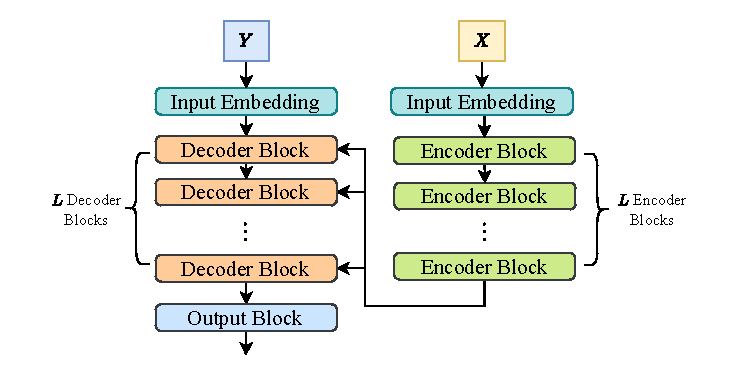
\includegraphics[width=1\linewidth]{fig/transformer.pdf}
    \caption{The transformer architecture, a closer look. Note that $L=6$ in the original paper \cite{vaswani2017attention}.}
    \label{fig:transformer}
\end{figure}

\printbibliography

\end{document}